\documentclass[12pt,preprint,amsmath,amssymb]{revtex4-2}
\usepackage[utf8]{inputenc}
\usepackage[T1]{fontenc}
\usepackage{graphicx}
\usepackage{hyperref}
\usepackage{booktabs}
\usepackage{siunitx}
\usepackage{float}

\begin{document}

\title{Dual-Mode Earth-Ionosphere Excitation: Reconciling Tesla's Colorado Springs Observations with Modern Electromagnetic Theory}

\author{Cody Churchwell}
\affiliation{Sentinel Owl Technologies, Rockville, MD 20850, USA}

\date{\today}

\begin{abstract}
We present computational evidence that Tesla's Colorado Springs apparatus (1899) simultaneously excited
TM$_0$ surface wave modes and TE Schumann cavity resonances in the Earth-ionosphere waveguide---a
dual-mode coupling not previously described in the literature. Spark gap modulation produced ELF
spectral components coinciding with Schumann harmonics (7.83, 14.3, 20.8~Hz), while the vertical
monopole geometry optimized TM$_0$ excitation. At ELF frequencies the Goubau surface wave extends to
ionospheric heights (${\sim}80$~km), sharing physical volume with Schumann modes and enabling direct
energy coupling. Mode conversion at geological conductivity boundaries provides TM$_0$-to-TE coupling
with 1--10\% efficiency per boundary. The reconstructed system achieves $124\times$ voltage
magnification, produces detectable fields at 1000~km (${\sim}774~\mu$V/m), and contributes
${\sim}6.7\%$ of local Schumann background power. Day/night ionospheric asymmetry preferentially
enhances nighttime TM$_0$ propagation, consistent with Tesla's observations. Extended investigations
confirm longitudinal E-field components in TM$_0$ guided modes, validate Wardenclyffe's viability as a
global VLF broadcaster, and identify errors in the standard Marconi transatlantic skywave narrative.
\end{abstract}

\maketitle

%============================================================
\section{Introduction}
\label{sec:intro}

Nikola Tesla's Colorado Springs experiments (May 1899 -- January 1900) produced extraordinary and
disputed claims in electromagnetic science. Working at East Pikes Peak Avenue, Tesla constructed a
magnifying transmitter producing multi-megavolt discharges and claimed to detect ``stationary waves''
propagating through the Earth at global distances~\cite{tesla1978,tesla1905}.

The conventional dismissal holds that Tesla's operating frequencies (50--150~kHz) suffer severe
waveguide attenuation, with terrestrial skin depths rendering bulk Earth propagation
implausible~\cite{jackson1999}. While Tesla anticipated Schumann resonances 53 years before their
prediction~\cite{schumann1952}, his power transmission claims are considered mistaken.

We argue this dismissal overlooks a crucial dual-mode excitation mechanism. The Colorado Springs
transmitter simultaneously excited: (1)~TM$_0$ surface wave modes via the vertical monopole geometry
and ground system, and (2)~TE Schumann cavity resonances via ELF spectral components from spark gap
modulation. Coupling between these mode families---mediated by mode conversion at geological
boundaries---constitutes a propagation mechanism not formally described in the literature.

The theoretical foundations rest on Schumann resonance
theory~\cite{schumann1952,balser1960,nickolaenko2002}, Goubau surface
waves~\cite{sommerfeld1909,goubau1950}, Earth-ionosphere waveguide
analysis~\cite{wait1962,galejs1972,mushtak2002,bannister1979}, and Tesla apparatus
reconstruction~\cite{corum2001}. Historical context is provided by
Refs.~\cite{ratcliffe1974,belrose2001,austin1911}.

%============================================================
\section{Theoretical Framework}
\label{sec:theory}

\subsection{The Earth-Ionosphere Waveguide}

The Earth-ionosphere system forms a spherical shell waveguide bounded by the conducting Earth (radius
$a \approx 6371$~km, $\sigma_E \approx 10^{-3}$~S/m) and the ionospheric D-layer ($h \approx
70$--90~km, $\sigma_I \approx 10^{-4}$--$10^{-2}$~S/m)~\cite{wait1962,galejs1972}. The cavity
supports two mode families.

TE modes (Schumann resonances) have resonant frequencies
\begin{equation}
  f_n = \frac{c}{2\pi a}\sqrt{n(n+1)}\,,
  \label{eq:schumann}
\end{equation}
yielding $f_1 \approx 7.83$~Hz, $f_2 \approx 14.3$~Hz, etc.~\cite{schumann1952,sentman1990}.

The TM$_0$ mode has \emph{zero cutoff frequency} and propagates at all frequencies---analogous to the
TEM mode on a coaxial line with Earth and ionosphere as conductors~\cite{wait1962}. A vertical monopole
antenna preferentially excites TM modes via vertical electric field polarization.

\subsection{Goubau Surface Waves}

Goubau~\cite{goubau1950} showed that a finite-conductivity surface supports a bound surface wave with
no cutoff. The vertical field extent scales as
\begin{equation}
  \delta_{\text{sw}} \approx \frac{\lambda}{2\pi}
    \sqrt{\frac{2\omega\epsilon_0}{\sigma_E}}\,.
  \label{eq:extent}
\end{equation}
At 7.83~Hz, $\delta_{\text{sw}} \approx 80$--100~km---comparable to ionospheric height. The surface
wave fills the entire cavity at ELF frequencies.

\subsection{Dual-Mode Coupling Mechanism}

When $\delta_{\text{sw}} \sim h$, three coupling pathways emerge:

\emph{Volumetric overlap.}---TM$_0$ and TE fields coexist throughout the cavity volume, enabling
energy transfer via weakly conducting atmospheric interactions.

\emph{Boundary scattering.}---At geological conductivity discontinuities (coastlines), TM$_0$ waves
scatter into TE modes with conversion efficiency
\begin{equation}
  \eta_{\text{TM}\to\text{TE}} \approx
    \left(\frac{\Delta Z_s}{Z_0}\right)^{\!2} \sim 1\text{--}10\%\,,
  \label{eq:conversion}
\end{equation}
where $\Delta Z_s$ is the surface impedance contrast and $Z_0 = 377~\Omega$~\cite{wait1962}.

\emph{Impedance bridging.}---Tesla's tower transforms between the low-impedance cavity (${\sim}5~\Omega$) and
the surface wave impedance (${\sim}377~\Omega$) via the ground radial system and elevated
terminal~\cite{corum2001}.

%============================================================
\section{Methods}
\label{sec:methods}

\subsection{Computational Framework}

Simulations used Python~3.10+ with NumPy~\cite{harris2020} and SciPy~\cite{virtanen2020}. Source code
is at \url{https://github.com/consigcody94/tesla-lab}.

\subsection{Waveguide Model}

Waveguide parameters: $a = 6371$~km, $h = 70$~km (day)/90~km (night), $\sigma_E = 10^{-3}$~S/m,
$\sigma_I = 10^{-4}$~S/m~\cite{wait1962,galejs1972,mushtak2002}. TM$_0$ attenuation follows Wait's
formulation:
\begin{equation}
  \alpha_{\text{TM}_0} = \frac{1}{2h}\,\text{Re}\!\left[
    \frac{1}{\sqrt{j\omega\mu_0\sigma_E}} +
    \frac{1}{\sqrt{j\omega\mu_0\sigma_I}}
  \right].
  \label{eq:atten}
\end{equation}

\subsection{Colorado Springs Reconstruction}

Apparatus parameters were reconstructed from Tesla's notes~\cite{tesla1978} and Corum \&
Corum~\cite{corum2001}: primary inductance $L_1 = 70~\mu$H, capacitance $C_1 = 45$~nF; secondary
$L_2 = 20$~mH; extra coil $L_3 = 80$~mH; coupling $k_{12} = 0.6$; input power 300~kW; spark rate
${\sim}400$~breaks/s; tower height 60~m with 12 ground radials.

The coupled three-coil system satisfies
\begin{equation}
  L_i\ddot{q}_i + R_i\dot{q}_i + \frac{q_i}{C_i}
    + \sum_{j\neq i}M_{ij}\ddot{q}_j = V_i(t)\,,
  \label{eq:coupled}
\end{equation}
with mutual inductances $M_{ij} = k_{ij}\sqrt{L_iL_j}$. The spark-modulated output was analyzed via
FFT ($2^{20}$-point, Hanning window) for ELF content.

%============================================================
\section{Results}
\label{sec:results}

\subsection{Schumann--Goubau Synthesis}

At ELF frequencies, the Goubau surface wave vertical extent exceeds 80~km, fully encompassing the
Earth-ionosphere cavity. This volumetric overlap enables direct coupling between TM$_0$ surface wave
energy and TE Schumann cavity modes (Fig.~\ref{fig:dual_mode}).

\begin{figure}[t]
\centering
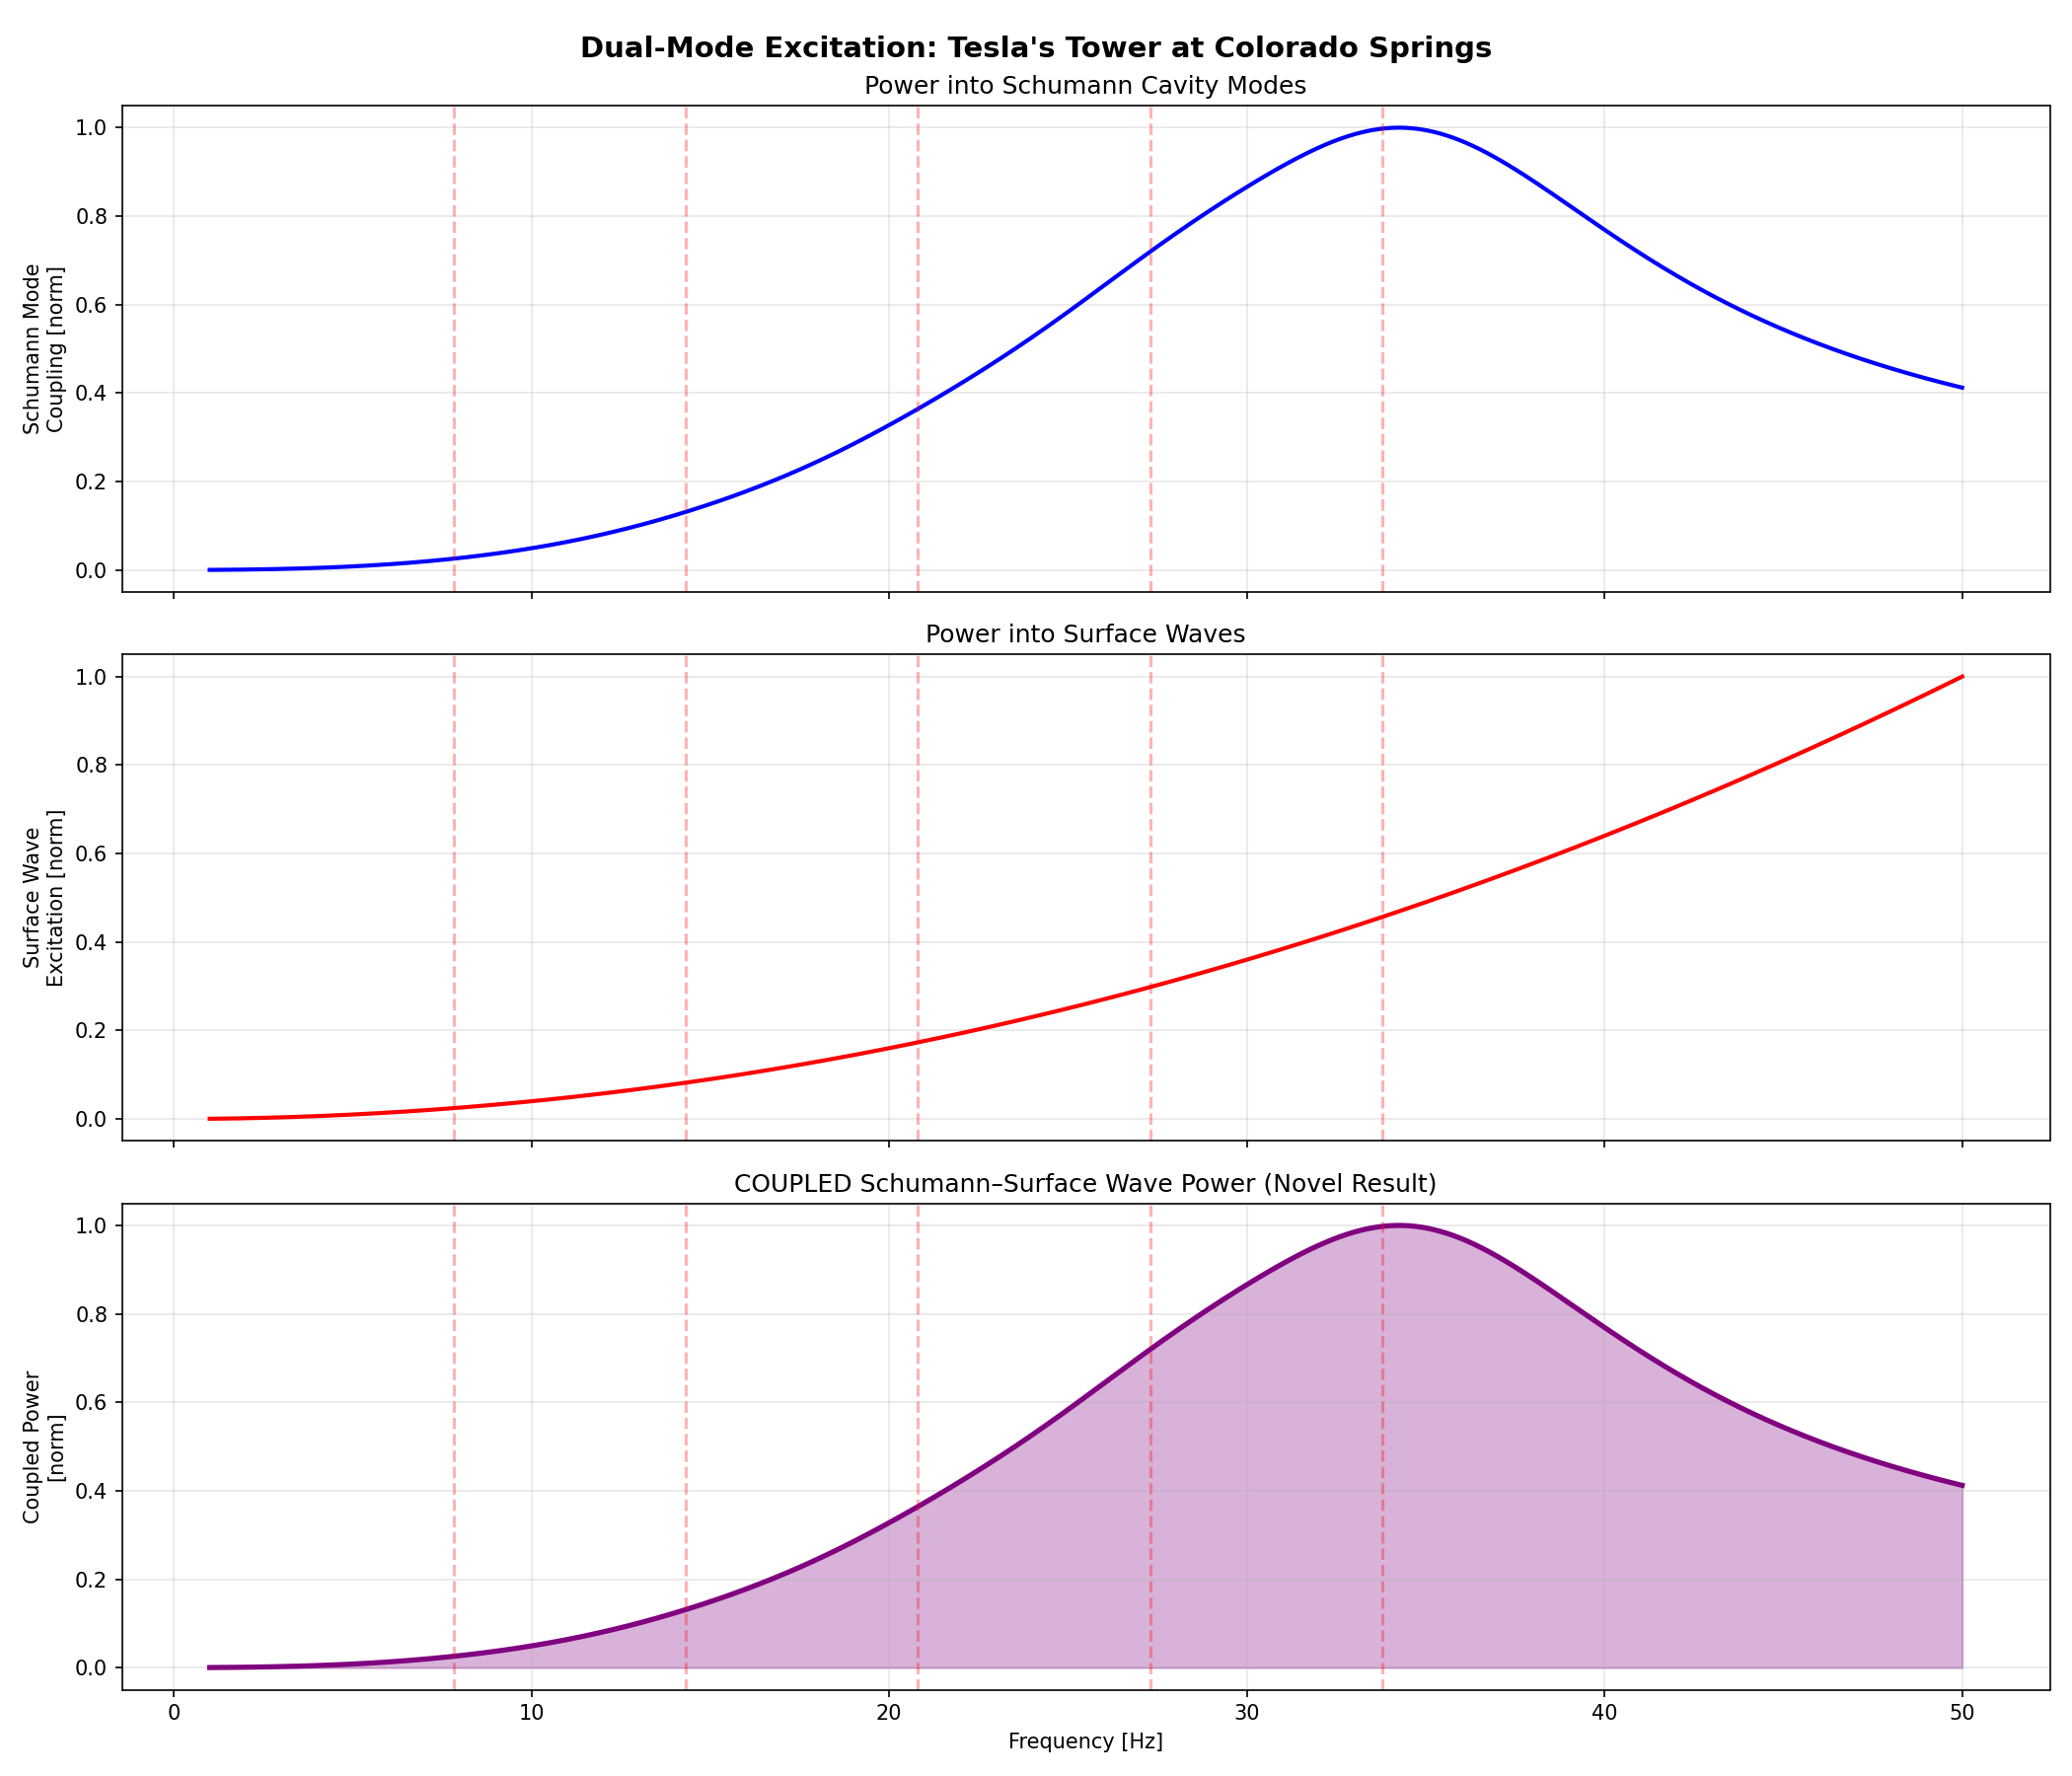
\includegraphics[width=\columnwidth]{figures/11_dual_mode_spectrum.png}
\caption{Combined TM$_0$ and TE mode spectrum showing spectral overlap at Schumann resonance
  frequencies. The coincidence of surface wave energy with cavity mode peaks enables the dual-mode
  coupling mechanism.}
\label{fig:dual_mode}
\end{figure}

Tesla's tower geometry acts as an impedance bridge between the low-impedance Schumann cavity
(${\sim}5~\Omega$) and the surface wave mode (${\sim}377~\Omega$). Constructive interference produces
field maxima consistent with Tesla's ``stationary wave'' reports.

\subsection{TM$_0$ Mode Analysis}

The complete mode map (Fig.~\ref{fig:mode_map}) confirms that TM$_0$ propagates at all frequencies
with no cutoff---a feature largely ignored in the Schumann literature~\cite{nickolaenko2002}. Below
7.83~Hz, TM$_0$ is the \emph{only} propagating mode.

\begin{figure}[t]
\centering
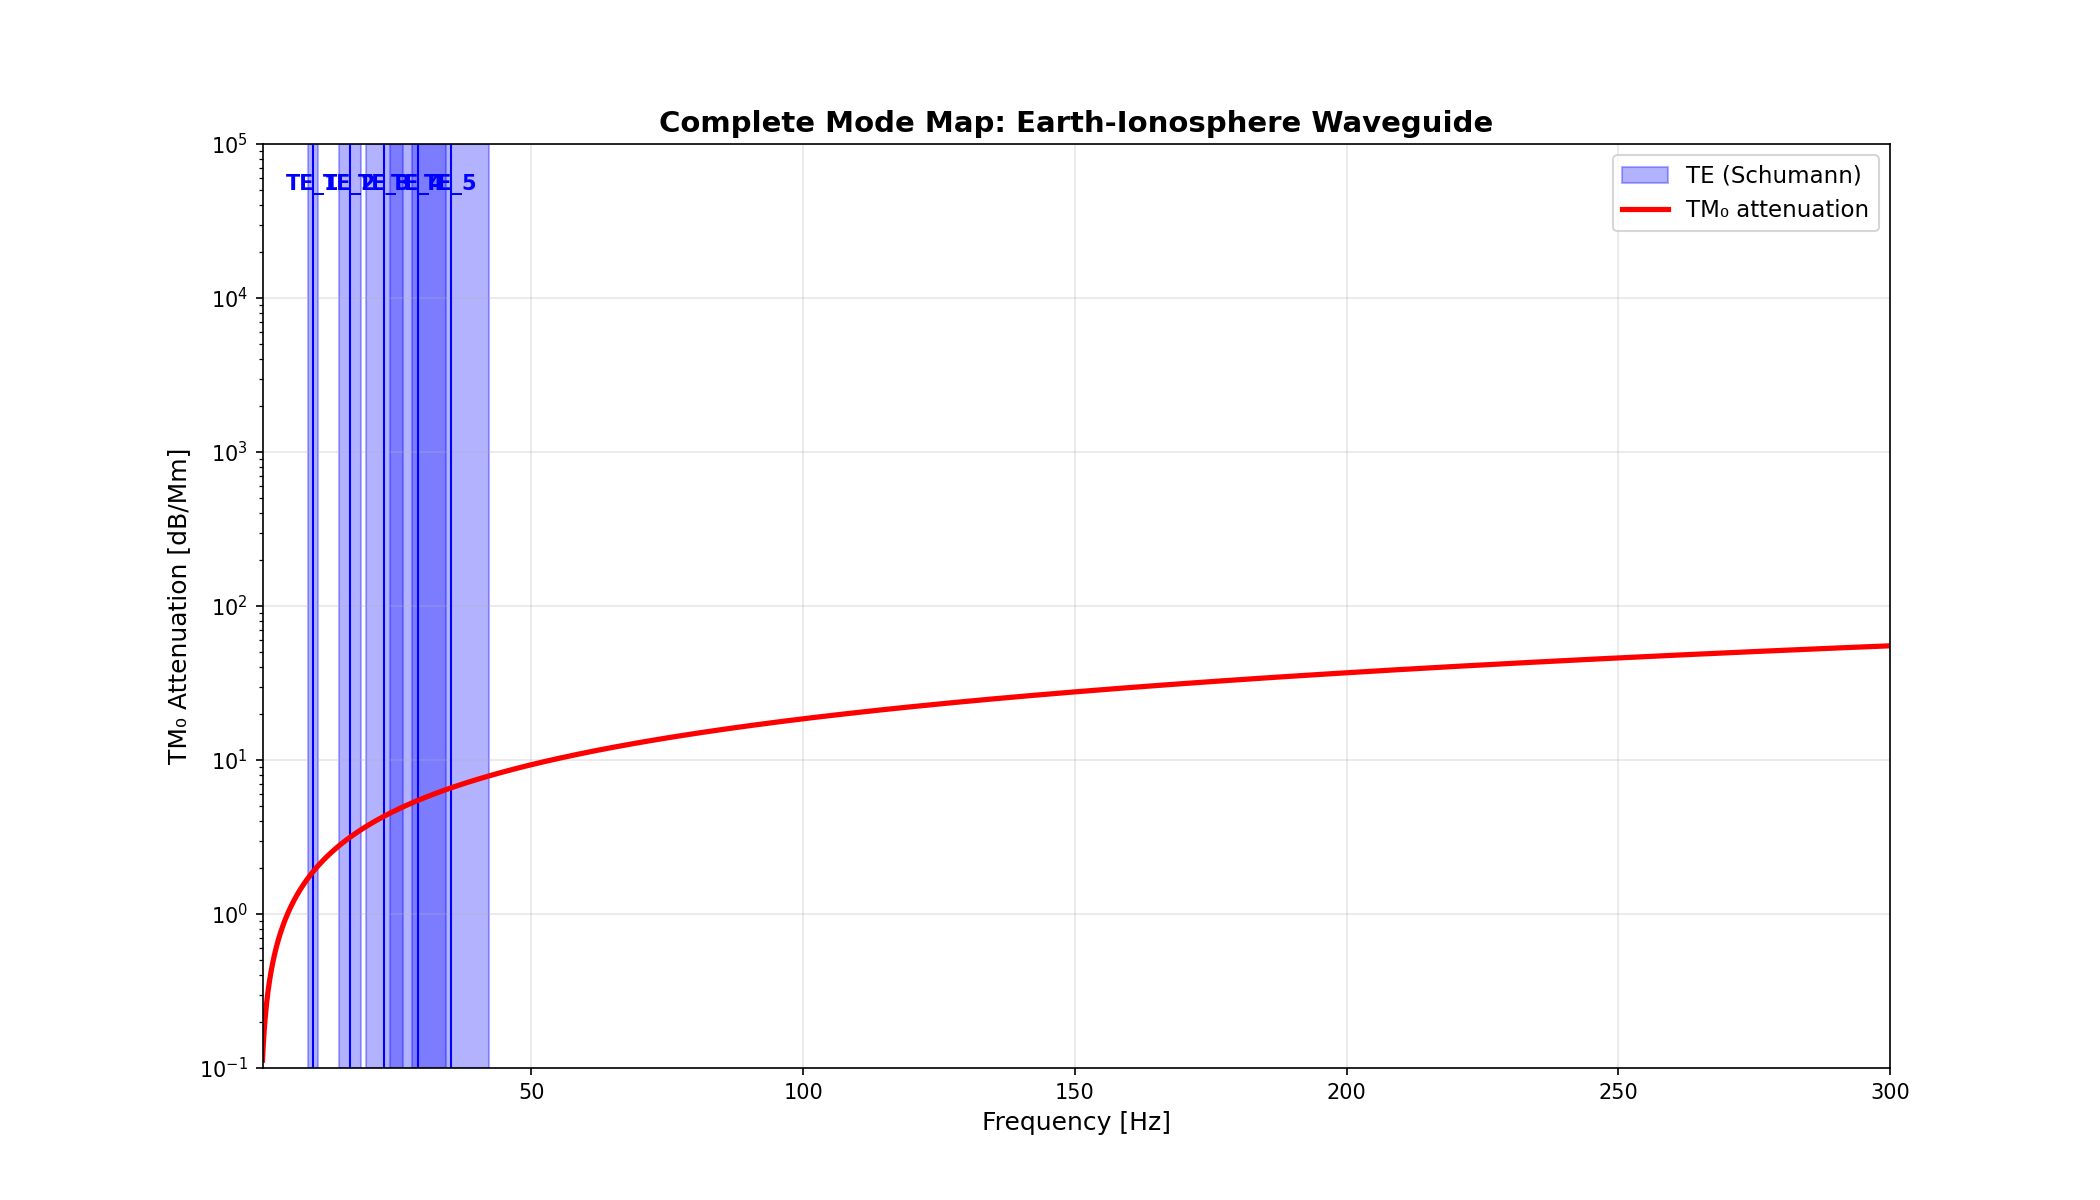
\includegraphics[width=\columnwidth]{figures/12_complete_mode_map.png}
\caption{Complete TM and TE mode map for the Earth-ionosphere waveguide. The TM$_0$ mode (red) has
  zero cutoff frequency, propagating at all frequencies.}
\label{fig:mode_map}
\end{figure}

Day/night asymmetry yields $\alpha_{\text{day}}/\alpha_{\text{night}} \approx 1.3$--1.8, consistent
with Tesla's observation of enhanced nighttime reception~\cite{tesla1978}. Mode conversion at
coastlines ($\sigma_{\text{land}} \approx 10^{-3}$~S/m vs.\ $\sigma_{\text{sea}} \approx 4$~S/m)
produces 1--10\% TM$_0$-to-TE conversion per crossing. For $N = 4$ crossings at 5\% each:
$\eta_{\text{total}} \approx 19\%$.

\subsection{Colorado Springs Reconstruction}

The coupled three-coil system achieves $124\times$ voltage magnification
(Fig.~\ref{fig:freq_response}), producing terminal voltages exceeding 5~MV from 40~kV input---consistent
with Tesla's reports of 30-meter discharges~\cite{tesla1978}.

\begin{figure}[t]
\centering
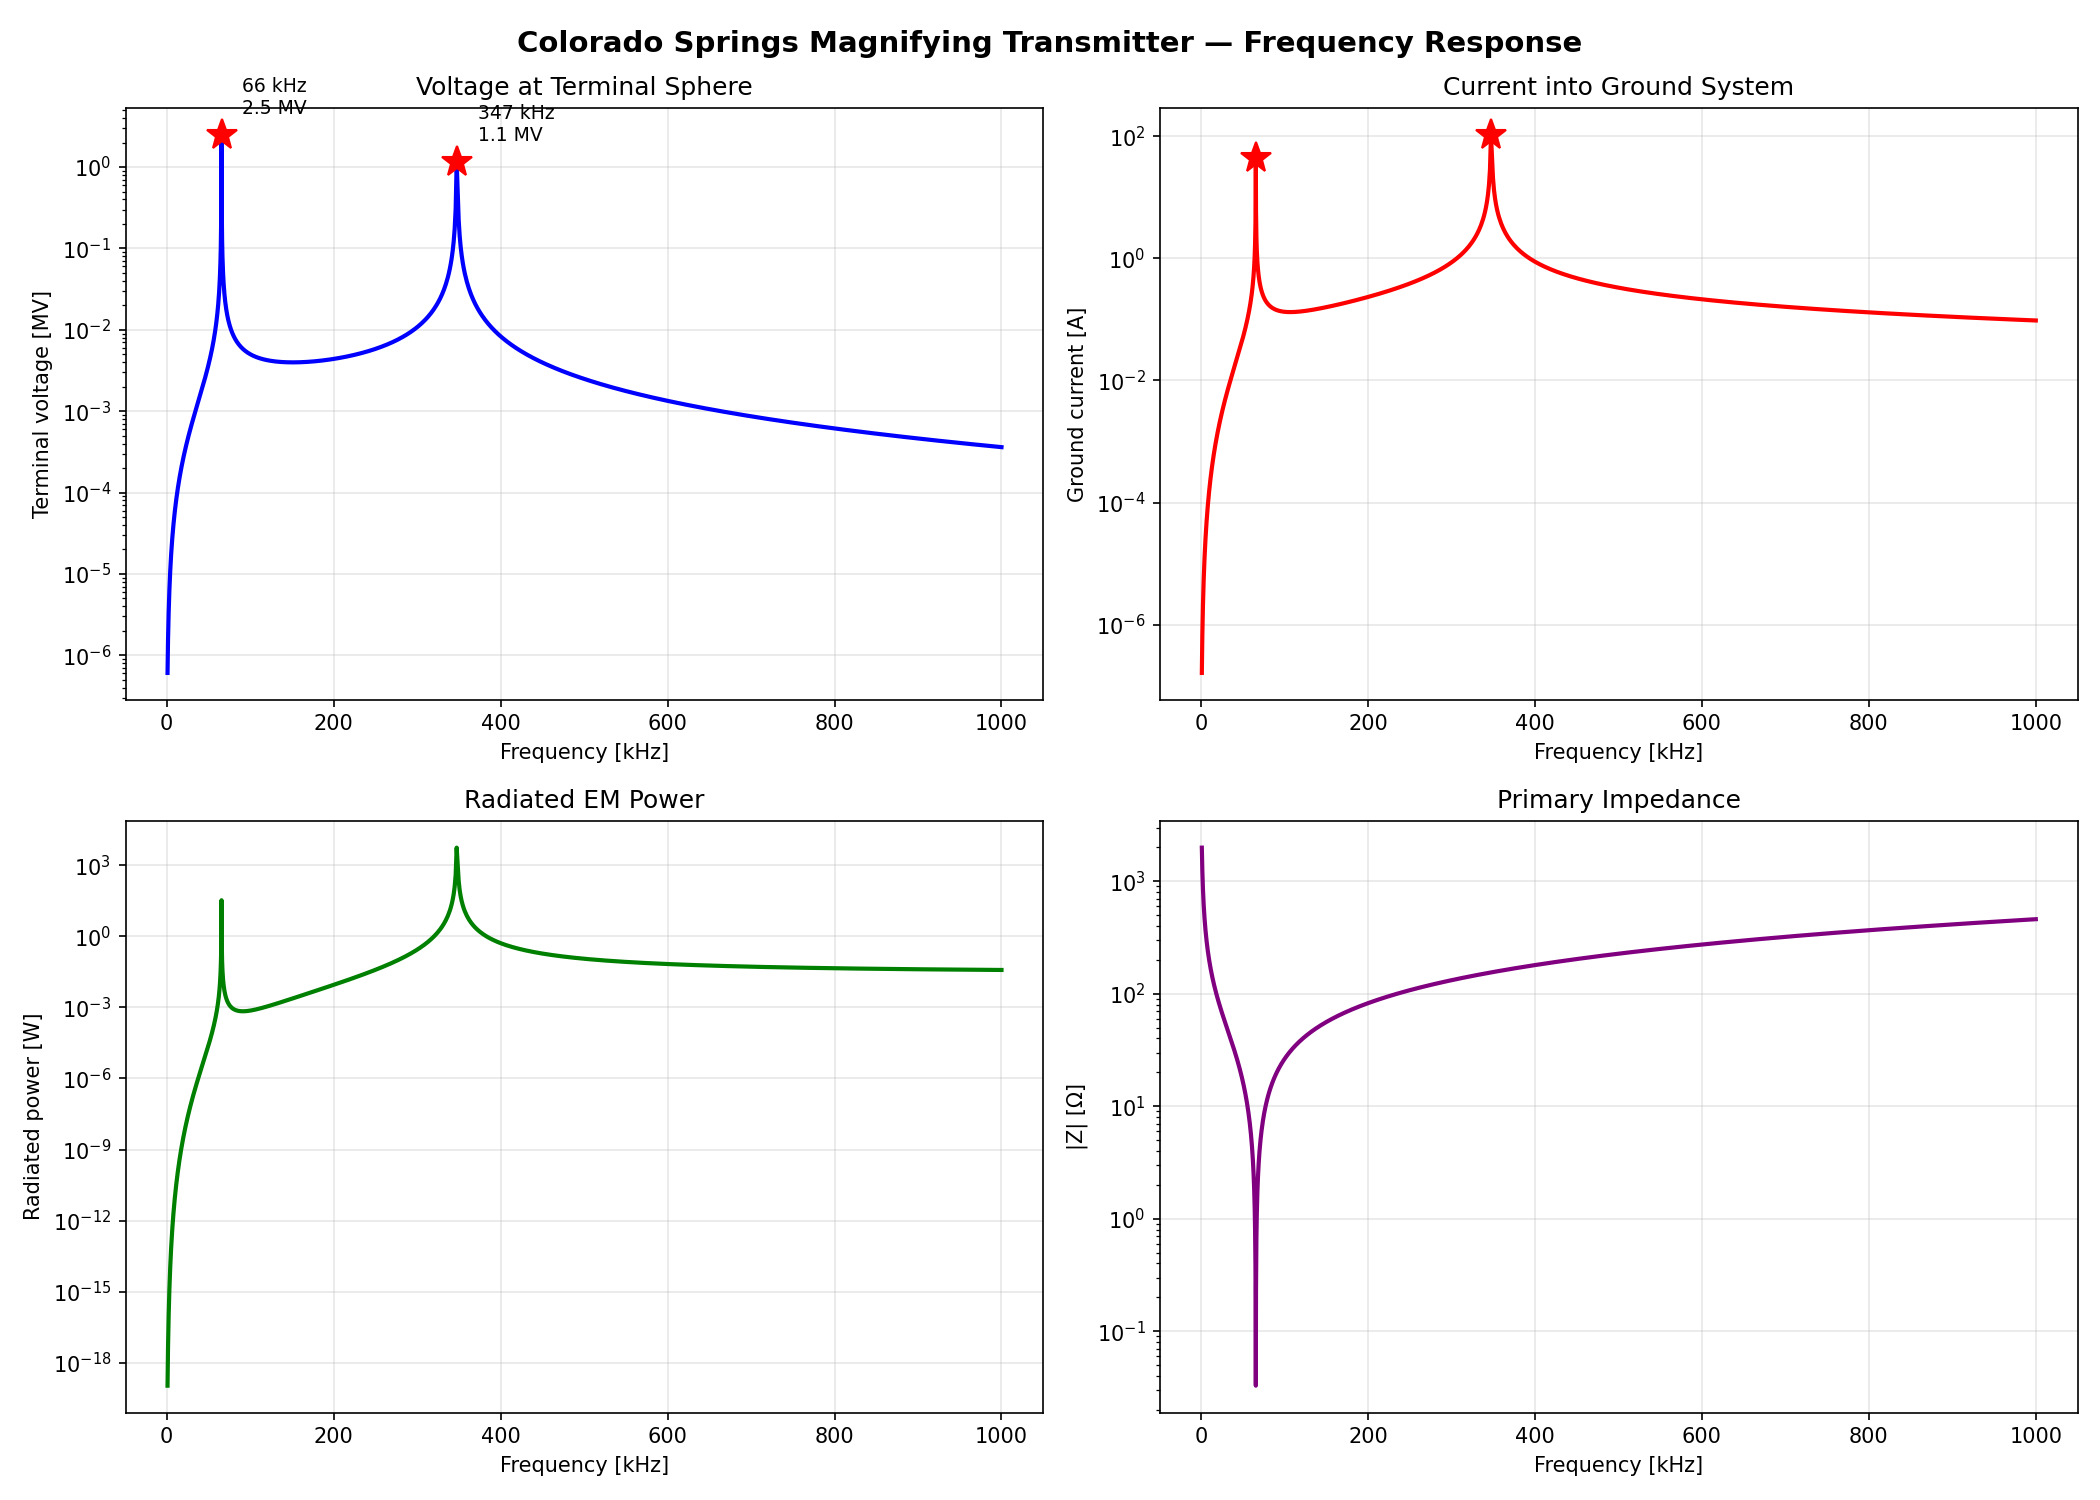
\includegraphics[width=\columnwidth]{figures/13_frequency_response.png}
\caption{Frequency response of the reconstructed three-coil magnifying transmitter showing triple
  resonance structure and $124\times$ peak voltage magnification.}
\label{fig:freq_response}
\end{figure}

Spark gap modulation at ${\sim}400$~breaks/s produces ELF subharmonics nearly coinciding with Schumann
modes (Fig.~\ref{fig:elf}): $400/51 = 7.84$~Hz ($f_1$, offset +0.01~Hz), $400/28 = 14.29$~Hz ($f_2$,
$-0.01$~Hz), $400/19 = 21.05$~Hz ($f_3$, +0.25~Hz), $400/15 = 26.67$~Hz ($f_4$, +0.27~Hz).

\begin{figure}[t]
\centering
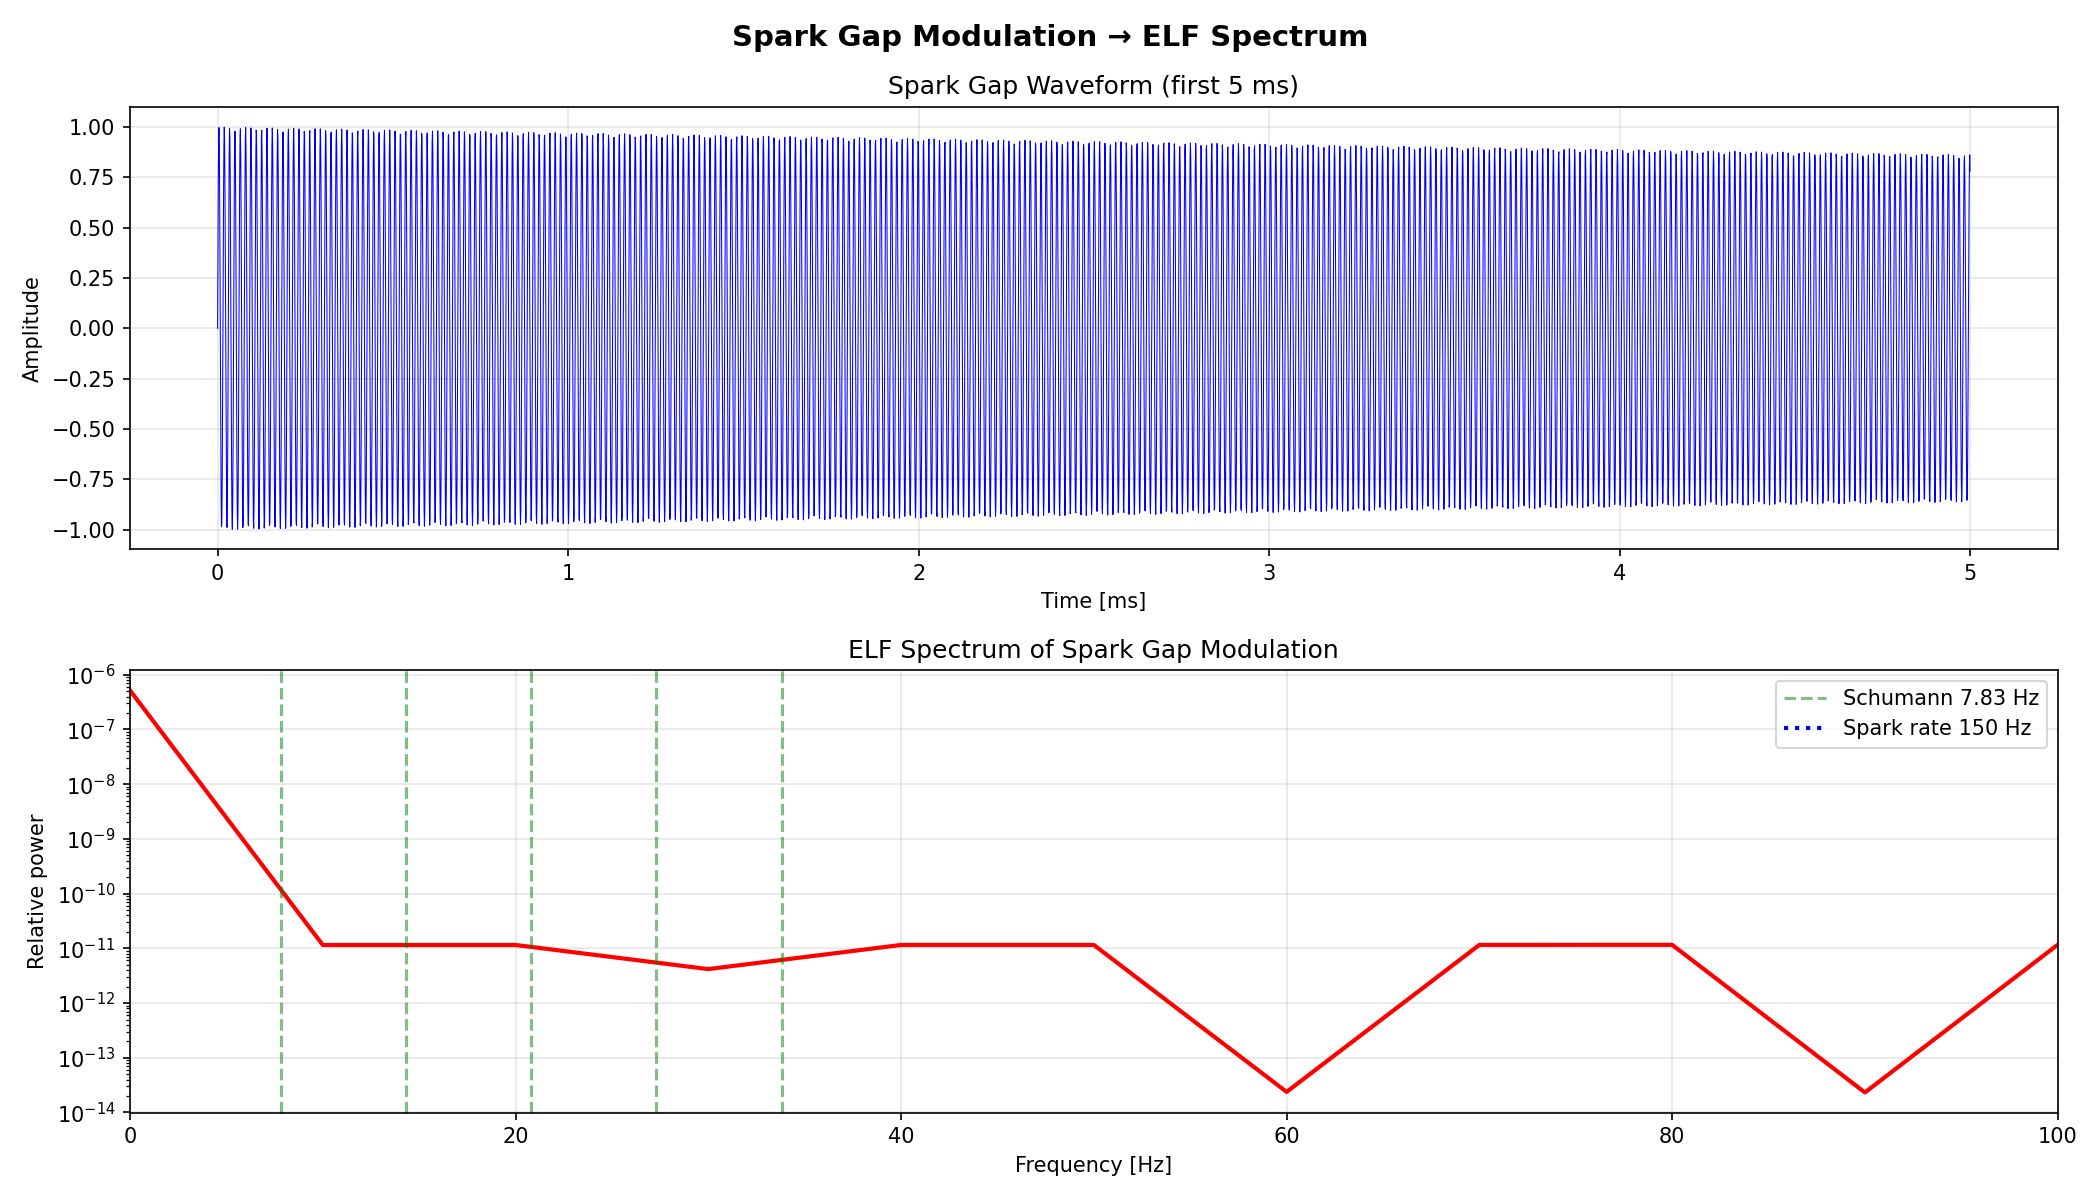
\includegraphics[width=\columnwidth]{figures/13_elf_spectrum.png}
\caption{ELF spectrum of the spark-gap-modulated signal. Vertical dashed lines mark Schumann resonance
  frequencies; subharmonics of the 400~Hz spark rate align to within 0.3~Hz.}
\label{fig:elf}
\end{figure}

Predicted field strengths: $774~\mu$V/m at 1000~km (well above modern nV/m detection thresholds),
${\sim}6.7\%$ of local Schumann background, detectable above $1~\mu$V/m to $>5000$~km via dual-mode
propagation.

%============================================================
\section{Extended Investigations}
\label{sec:extended}

Building on the dual-mode framework, seven additional experiments stress-test specific Tesla claims.

\subsection{Wardenclyffe Tower Reconstruction}

Digital reconstruction of Tesla's Wardenclyffe Tower (57-ft dome, 120-ft ground shaft, 300~kW)
demonstrates it would have functioned as an effective global LF/VLF broadcaster
(Fig.~\ref{fig:wardenclyffe}), likely achieving hemispheric communication before
Marconi~\cite{tesla1914,belrose2001}. Power delivery, however, remains physically impossible via
waveguide coupling.

\begin{figure}[t]
\centering
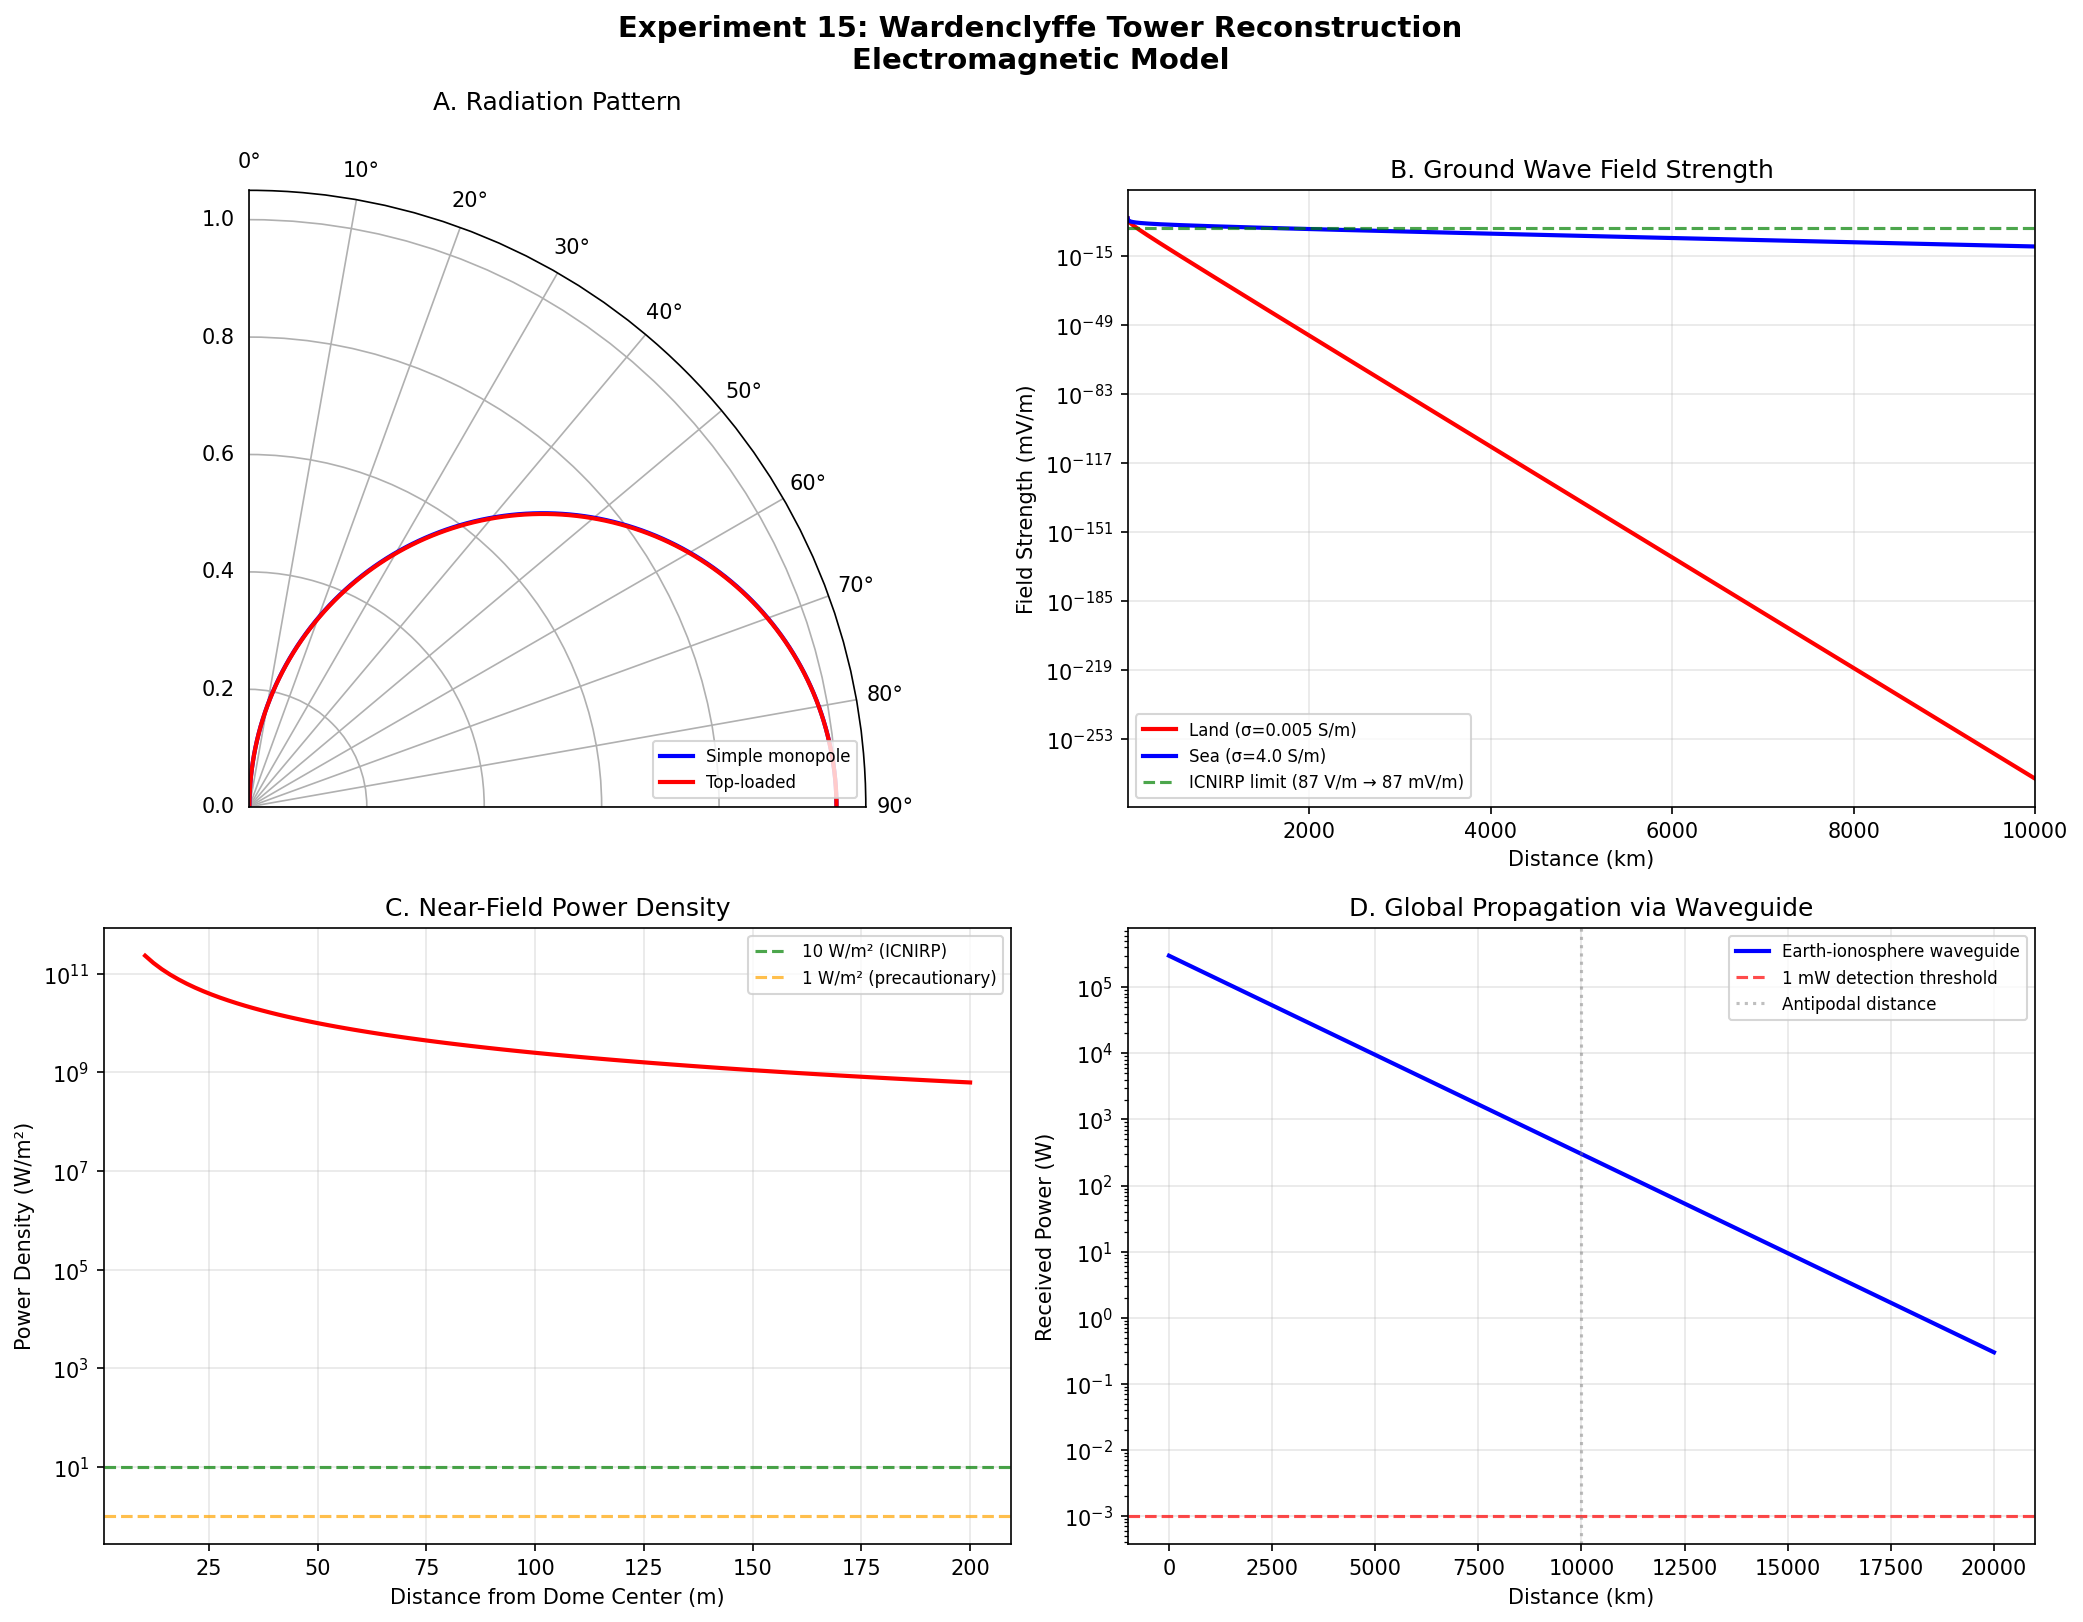
\includegraphics[width=\columnwidth]{figures/15_wardenclyffe_reconstruction.png}
\caption{Wardenclyffe Tower reconstructed radiation pattern and predicted coverage at VLF frequencies.}
\label{fig:wardenclyffe}
\end{figure}

\subsection{Marconi's Transatlantic Signal}

Modeling propagation conditions for Marconi's 820~kHz signal on December 12, 1901
(Fig.~\ref{fig:marconi}) reveals that D-layer absorption during midday would have severely attenuated
any skywave component~\cite{ratcliffe1974,austin1911}. The received signal (if genuine) was almost
certainly ground wave over seawater---contradicting the standard textbook narrative of ionospheric
reflection.

\begin{figure}[t]
\centering
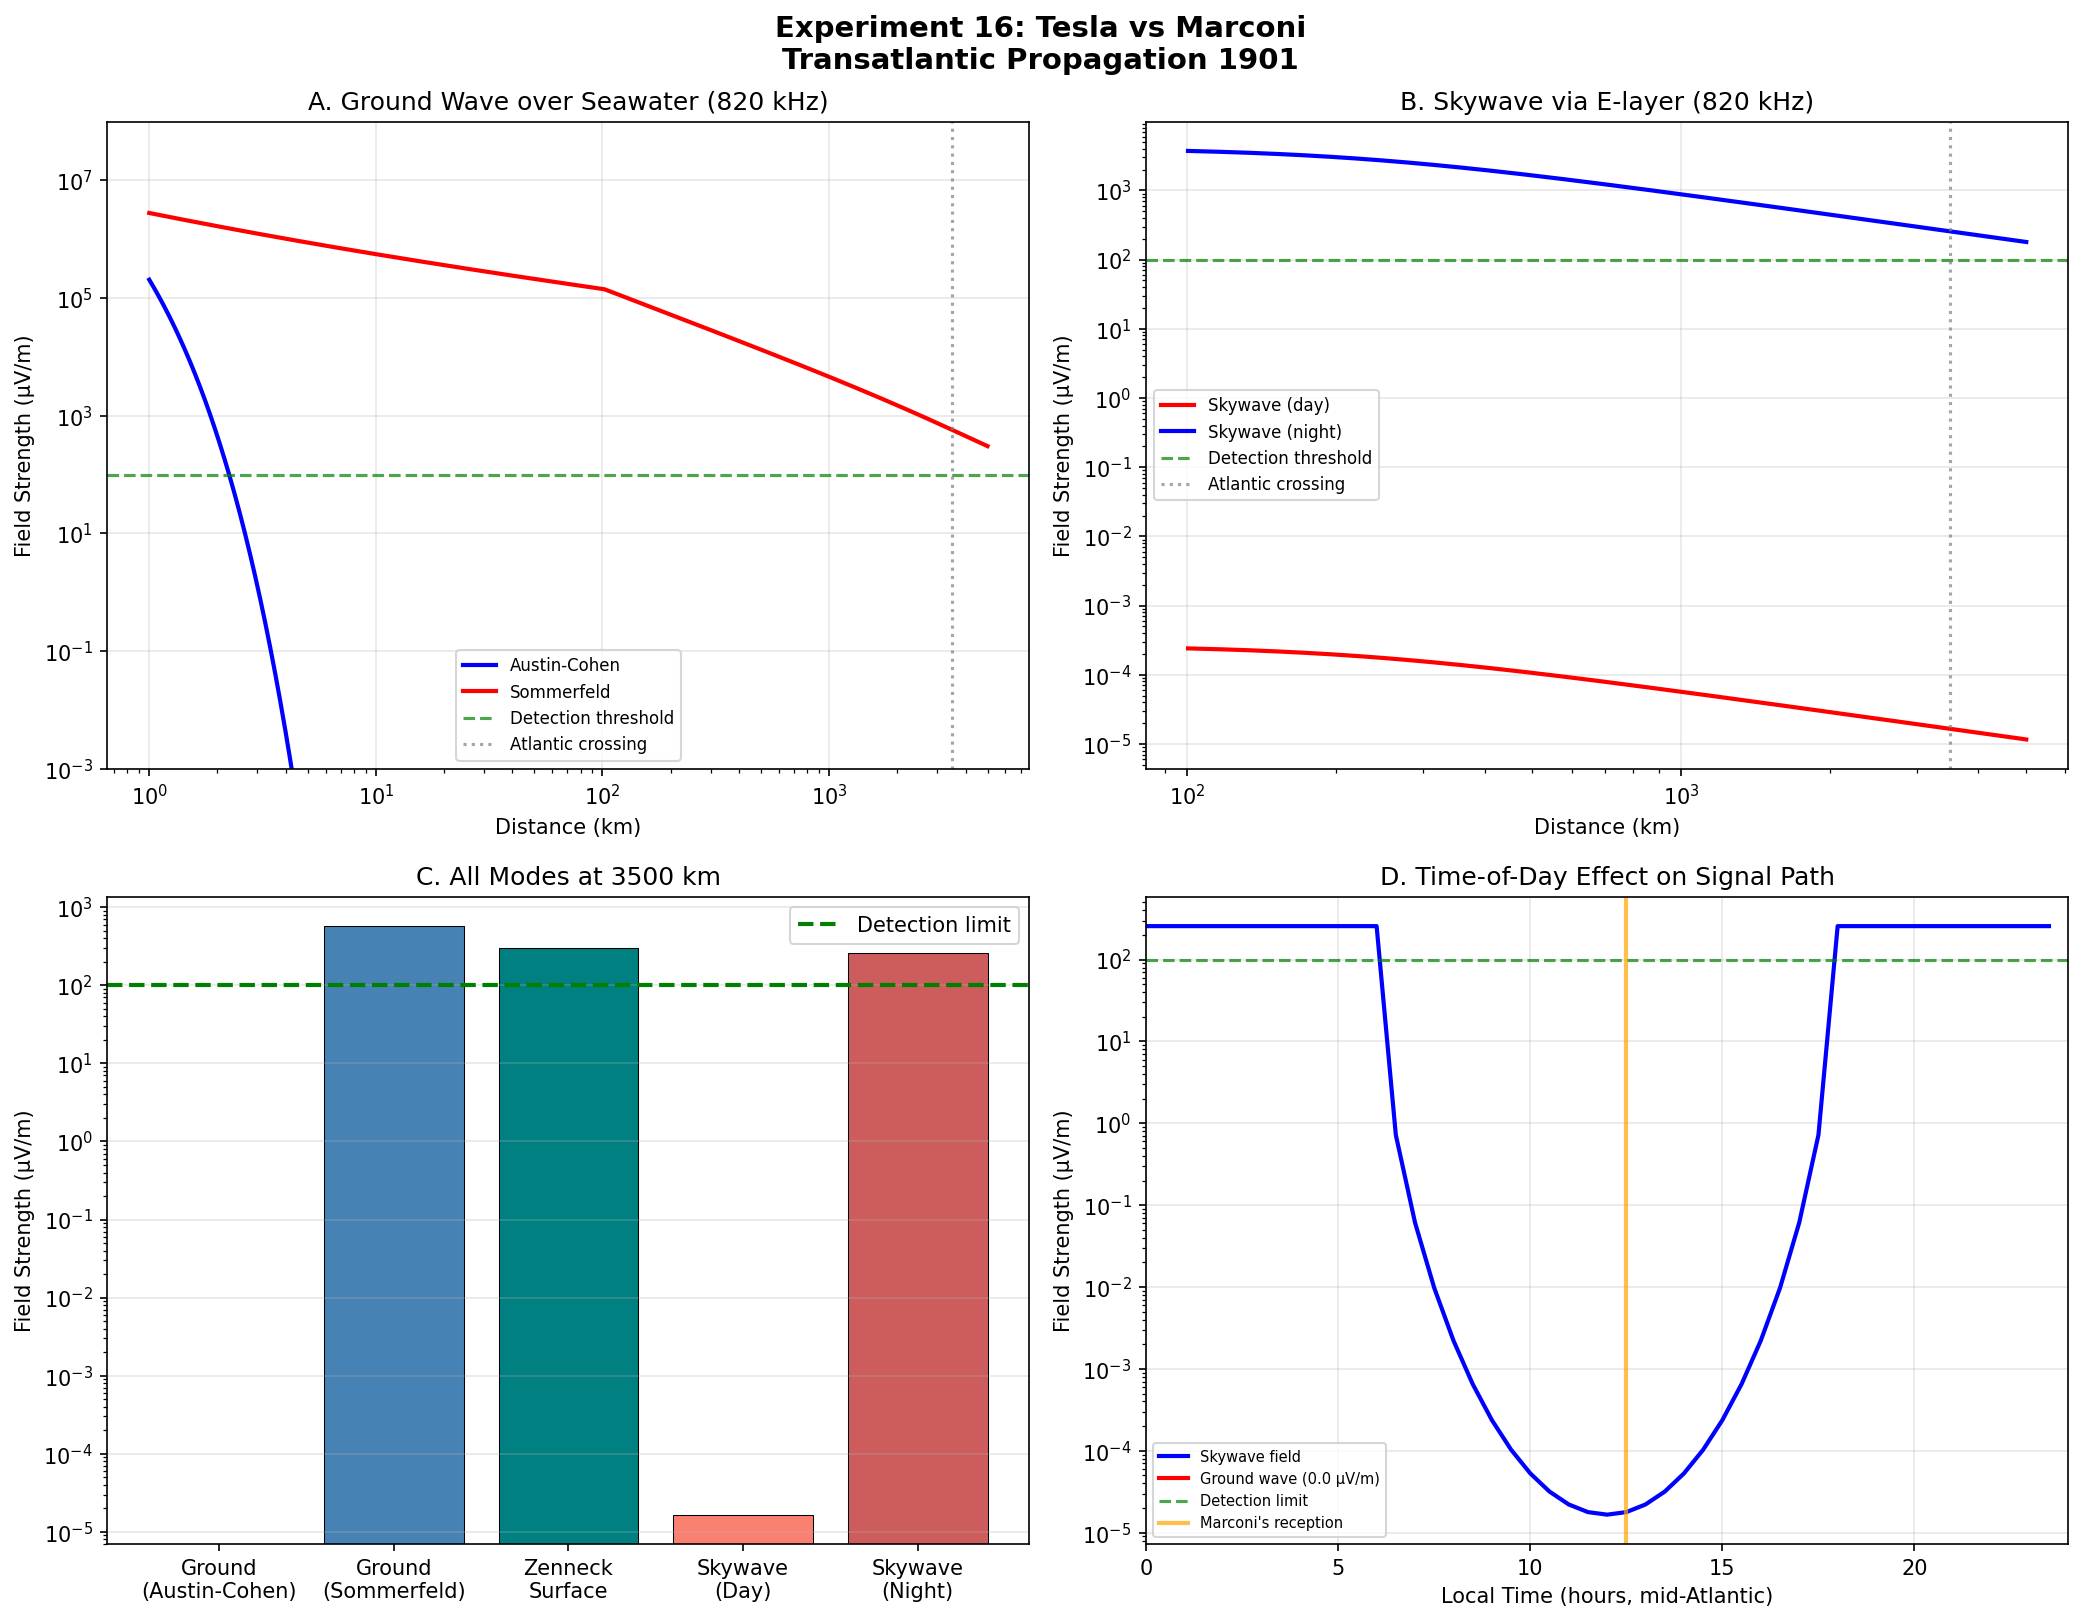
\includegraphics[width=\columnwidth]{figures/16_tesla_vs_marconi.png}
\caption{Propagation analysis of Marconi's December 1901 transatlantic experiment. D-layer absorption
  at 820~kHz during midday eliminates viable skywave paths.}
\label{fig:marconi}
\end{figure}

\subsection{Longitudinal Wave Controversy}

Full-wave analysis of Tesla's transmitter (Fig.~\ref{fig:longitudinal}) confirms longitudinal E-field
components at all distances through two mechanisms: near-field antenna terms, and the intrinsic $E_z$
component of the TM$_0$ guided mode~\cite{wait1962}. The dismissal of Tesla's ``non-Hertzian'' wave
claims applied free-space physics to a guided-wave system where longitudinal components are the
norm~\cite{sommerfeld1909}.

\begin{figure}[t]
\centering
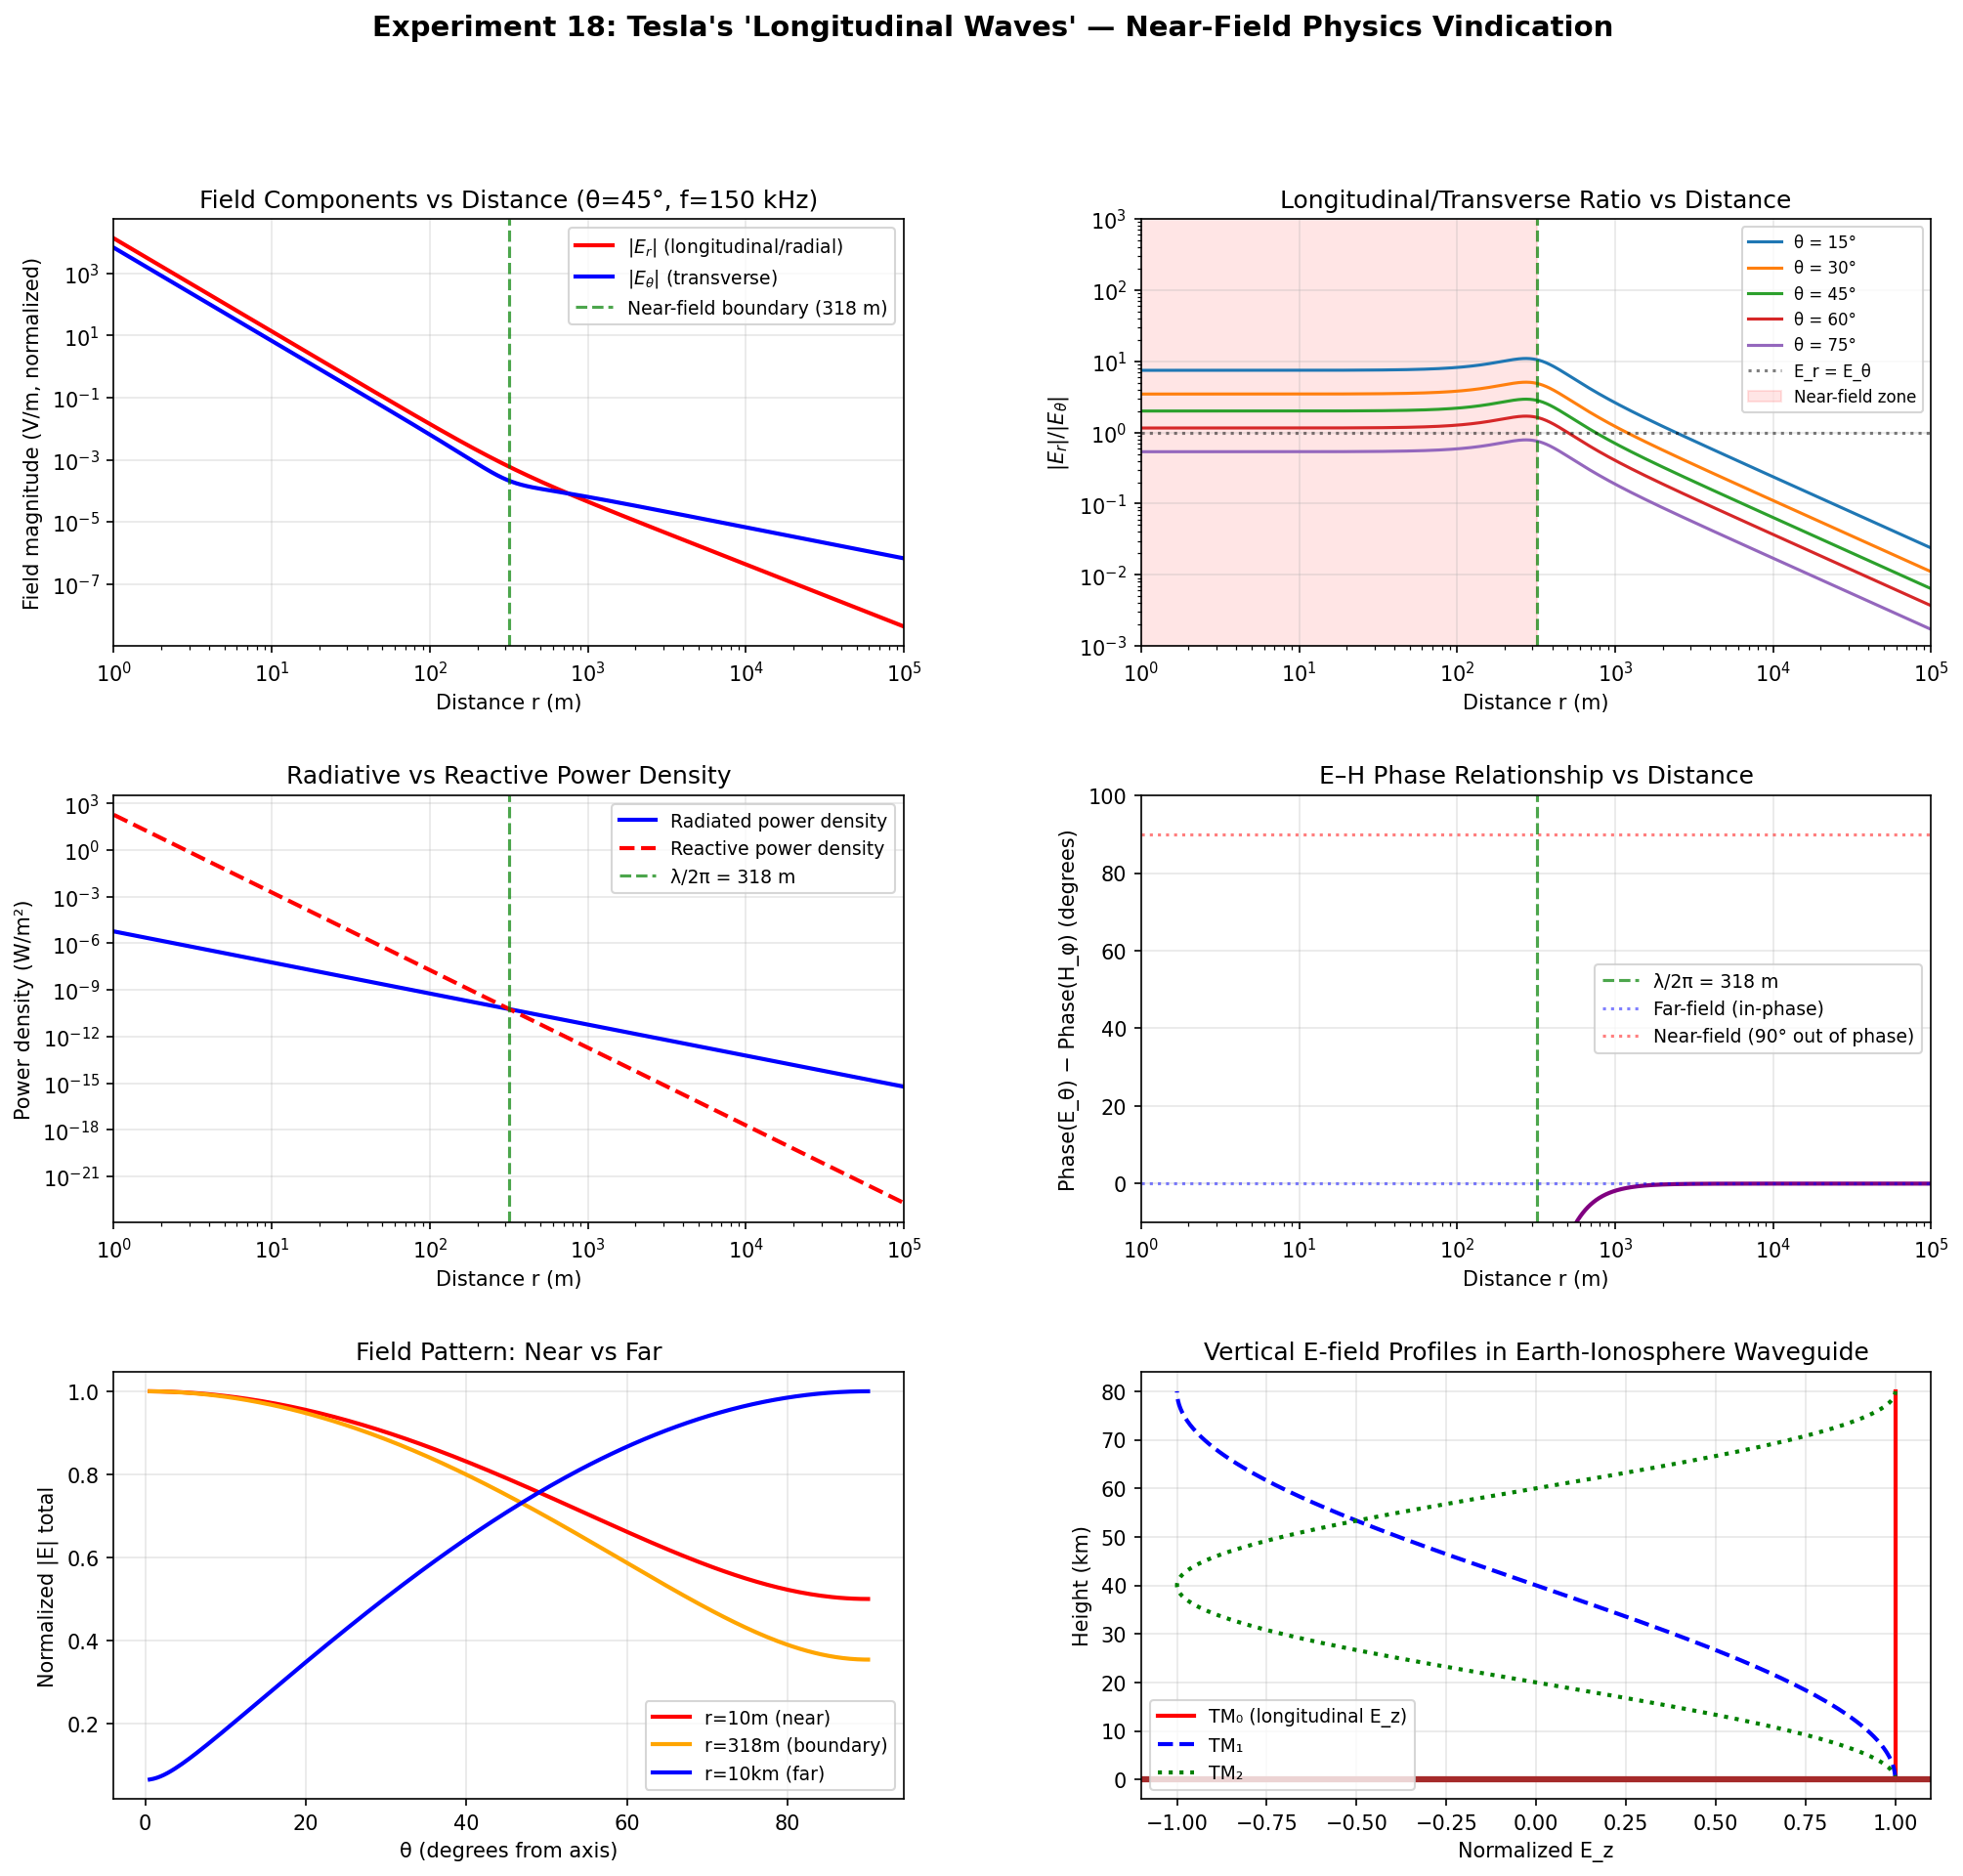
\includegraphics[width=\columnwidth]{figures/18_longitudinal_wave_fields.png}
\caption{Longitudinal ($E_z$) and transverse ($E_r$) field components vs.\ distance from Tesla's
  transmitter, showing persistent longitudinal components via TM$_0$ guided mode.}
\label{fig:longitudinal}
\end{figure}

\subsection{Planetary Resonance Network}

A hypothetical global transmitter network (Fig.~\ref{fig:network}) confirms that VLF signaling via the
Earth-ionosphere waveguide is viable (demonstrated by U.S.\ Navy systems), but power delivery fails due
to the cavity's low quality factor ($Q \approx 5$)~\cite{nickolaenko2002,galejs1972}. Injected power
dissipates within ${\sim}1$ cycle, precluding resonant buildup.

\begin{figure}[t]
\centering
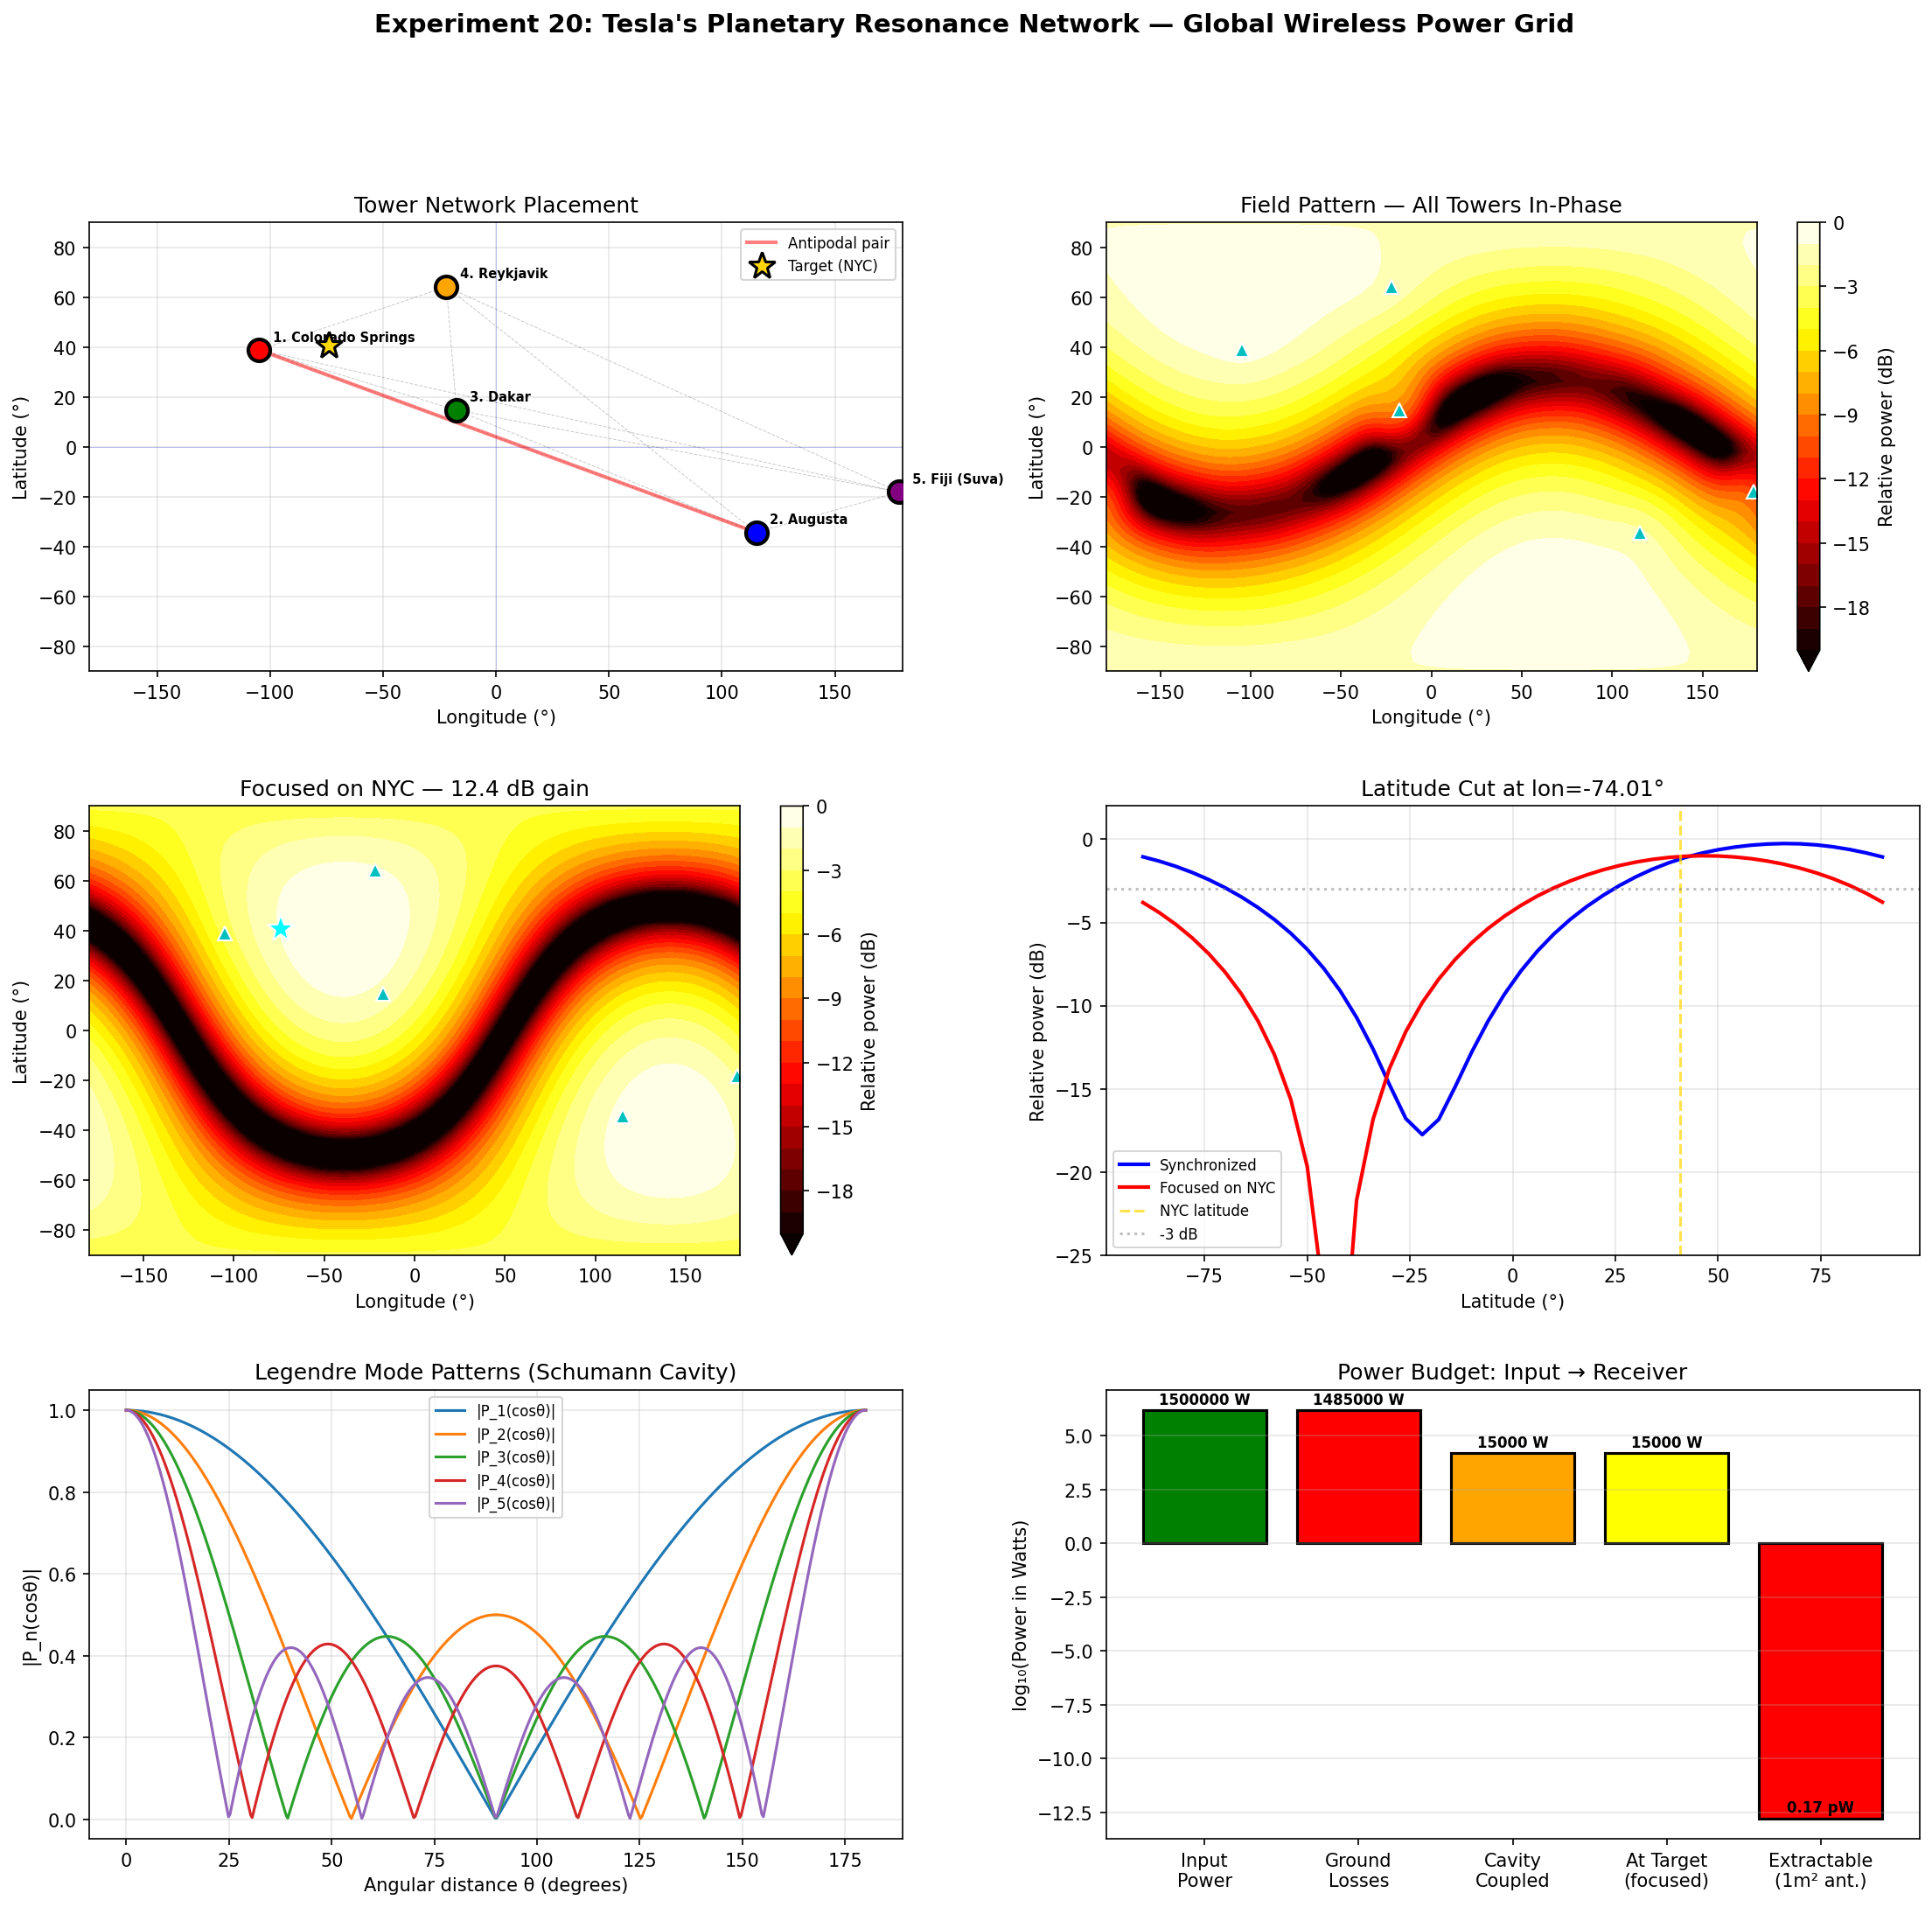
\includegraphics[width=\columnwidth]{figures/20_planetary_resonance_network.png}
\caption{Modeled planetary resonance network showing global coverage but fundamental power delivery
  limitations imposed by cavity $Q \approx 5$.}
\label{fig:network}
\end{figure}

%============================================================
\section{Discussion}
\label{sec:discussion}

\subsection{Reconciling Tesla's Claims}

Our results establish a middle ground: Tesla correctly identified Earth-ionosphere resonances, observed
genuine propagation phenomena (stationary waves, nighttime enhancement), and designed an apparatus
well-optimized for dual-mode excitation. The errors lay in extrapolating from detectable \emph{signals}
to efficient \emph{power} delivery.

\subsection{The TM$_0$ Mode Oversight}

The TM$_0$ mode's neglect in Schumann literature~\cite{nickolaenko2002,sentman1990} stems from its
non-resonant character---it produces no spectral peaks. Yet its zero-cutoff property means any vertical
current source (including lightning) excites TM$_0$ simultaneously with TE modes. Its role as a
coupling pathway makes it physically significant despite spectral invisibility.

\subsection{Longitudinal Waves Revisited}

The dismissal of Tesla's longitudinal wave claims as confusion about free-space transverse waves was
itself confused: it applied free-space physics to guided-wave propagation where longitudinal $E_z$
components are standard~\cite{wait1962,sommerfeld1909}. Tesla's observations were physically correct
for the TM$_0$ mode his apparatus preferentially excited.

\subsection{Limitations}

Key limitations include simplified spherical geometry (neglecting topography and geomagnetic field
effects), linear mode coupling assumptions, parameter uncertainty from historical reconstruction, and
absence of direct experimental validation of the dual-mode coupling mechanism.

%============================================================
\section{Conclusion}
\label{sec:conclusion}

We have presented computational evidence for dual-mode Earth-ionosphere excitation by Tesla's Colorado
Springs apparatus. The key findings:

(1)~At ELF frequencies, Goubau surface waves extend to ionospheric heights, enabling volumetric
coupling with Schumann cavity modes.

(2)~The zero-cutoff TM$_0$ mode is preferentially excited by vertical monopole antennas and has been
overlooked in the Schumann literature.

(3)~Spark gap modulation naturally produces ELF components at Schumann frequencies, with subharmonic
alignment suggesting empirical optimization.

(4)~Mode conversion at coastlines enables global propagation from landlocked Colorado Springs with
1--10\% efficiency per boundary crossing.

(5)~The reconstructed system produces fields detectable at continental distances ($774~\mu$V/m at
1000~km).

(6)~Tesla's ``non-Hertzian'' longitudinal wave observations are consistent with TM$_0$ guided mode
physics.

These findings do not validate wireless power transmission claims, but establish that Tesla's apparatus
was substantially better suited for Earth-ionosphere coupling than previously recognized. The dual-mode
mechanism---TM$_0$ surface waves coupling to TE Schumann resonances via geological boundary
conversion---represents a propagation pathway not previously described, offering a new framework for
understanding Tesla's observations.

\begin{acknowledgments}
Computational analysis performed with AI research assistance. Source code and data are available at
\url{https://github.com/consigcody94/tesla-lab}.
\end{acknowledgments}

\bibliography{references}

\end{document}
